\documentclass[a4paper, 12pt]{article}
\usepackage[utf8x]{inputenc}
\usepackage[T2A]{fontenc}
\usepackage[russian]{babel}
\usepackage[a4paper, left=30mm, right=15mm, top=20mm, bottom=20mm]{geometry}
\usepackage{booktabs}
\usepackage{tabu}
\usepackage[labelfont=bf, skip=5pt, font=small]{caption}
\usepackage{subcaption}
\usepackage{graphicx}
\usepackage{fancyhdr}
\usepackage{tocbibind}
\usepackage{indentfirst}
\usepackage{hyperref}
\usepackage{xcolor}
\usepackage{listings}

%New colors defined below
\definecolor{codegreen}{rgb}{0,0.6,0}
\definecolor{codegray}{rgb}{0.5,0.5,0.5}
\definecolor{codeorange}{rgb}{0.78, 0.564, 0}
\definecolor{backcolour}{rgb}{0.95,0.95,0.92}

%Code listing style named "mystyle"
\lstdefinestyle{mystyle}{
  backgroundcolor=\color{backcolour}, commentstyle=\color{codegreen},
  keywordstyle=\color{purple},
  numberstyle=\tiny\color{codegray},
  stringstyle=\color{codeorange},
  basicstyle=\ttfamily\footnotesize,
  breakatwhitespace=false,         
  breaklines=true,                 
  captionpos=b,                    
  keepspaces=true,                 
  numbers=left,                    
  numbersep=5pt,                  
  showspaces=false,                
  showstringspaces=false,
  showtabs=false,                  
  tabsize=2
}

%"mystyle" code listing set
\lstset{style=mystyle}
\lstset{
    inputencoding=utf8,        % Кодировка входного текста
    extendedchars=true,        % Включить поддержку расширенных символов
    literate={а}{{\char224}}1
             {б}{{\char225}}1
             {в}{{\char226}}1
             {г}{{\char227}}1
             {д}{{\char228}}1
             {е}{{\char229}}1
             {ё}{{\char184}}1
             {ж}{{\char230}}1
             {з}{{\char231}}1
             {и}{{\char232}}1
             {й}{{\char233}}1
             {к}{{\char234}}1
             {л}{{\char235}}1
             {м}{{\char236}}1
             {н}{{\char237}}1
             {о}{{\char238}}1
             {п}{{\char239}}1
             {р}{{\char240}}1
             {с}{{\char241}}1
             {т}{{\char242}}1
             {у}{{\char243}}1
             {ф}{{\char244}}1
             {х}{{\char245}}1
             {ц}{{\char246}}1
             {ч}{{\char247}}1
             {ш}{{\char248}}1
             {щ}{{\char249}}1
             {ъ}{{\char250}}1
             {ы}{{\char251}}1
             {ь}{{\char252}}1
             {э}{{\char253}}1
             {ю}{{\char254}}1
             {я}{{\char255}}1
             {А}{{\char192}}1
             {Б}{{\char193}}1
             {В}{{\char194}}1
             {Г}{{\char195}}1
             {Д}{{\char196}}1
             {Е}{{\char197}}1
             {Ё}{{\char168}}1
             {Ж}{{\char198}}1
             {З}{{\char199}}1
             {И}{{\char200}}1
             {Й}{{\char201}}1
             {К}{{\char202}}1
             {Л}{{\char203}}1
             {М}{{\char204}}1
             {Н}{{\char205}}1
             {О}{{\char206}}1
             {П}{{\char207}}1
             {Р}{{\char208}}1
             {С}{{\char209}}1
             {Т}{{\char210}}1
             {У}{{\char211}}1
             {Ф}{{\char212}}1
             {Х}{{\char213}}1
             {Ц}{{\char214}}1
             {Ч}{{\char215}}1
             {Ш}{{\char216}}1
             {Щ}{{\char217}}1
             {Ъ}{{\char218}}1
             {Ы}{{\char219}}1
             {Ь}{{\char220}}1
             {Э}{{\char221}}1
             {Ю}{{\char222}}1
             {Я}{{\char223}}1
}

\graphicspath{ {./img/} }

\setlength{\parskip}{1em}
\setlength{\parindent}{1.25cm}


\begin{document}

\thispagestyle{empty}
\begin{center}
    \textbf{Министерство науки и высшего образования Российской Федерации}\\
    ФЕДЕРАЛЬНОЕ ГОСУДАРСТВЕННОЕ АВТОНОМНОЕ ОБРАЗОВАТЕЛЬНОЕ УЧРЕЖДЕНИЕ ВЫСШЕГО ОБРАЗОВАНИЯ\\
    \textbf{НАЦИОНАЛЬНЫЙ ИССЛЕДОВАТЕЛЬСКИЙ УНИВЕРСИТЕТ ИТМО}\\[40pt]
    \textbf{Факультет безопасности информационных технологий}\\[40pt]
    \textbf{Дисциплина:}\\[10pt]
    «Техгологии и методы программирования»\\[30pt]
    \textbf{ОТЧЕТ ПО ЛАБОРАТОРНОЙ РАБОТЕ №5}\\[148pt]
\end{center}
\begin{flushright}
    \textbf{Выполнил:}\\[5pt]
    Михайлик Антон Денисович, студент группы N3351
    \begin{minipage}{0.7\textwidth}
        \hfill 
        \end{minipage}%
        \hfill
        \begin{minipage}{0.2\textwidth}
          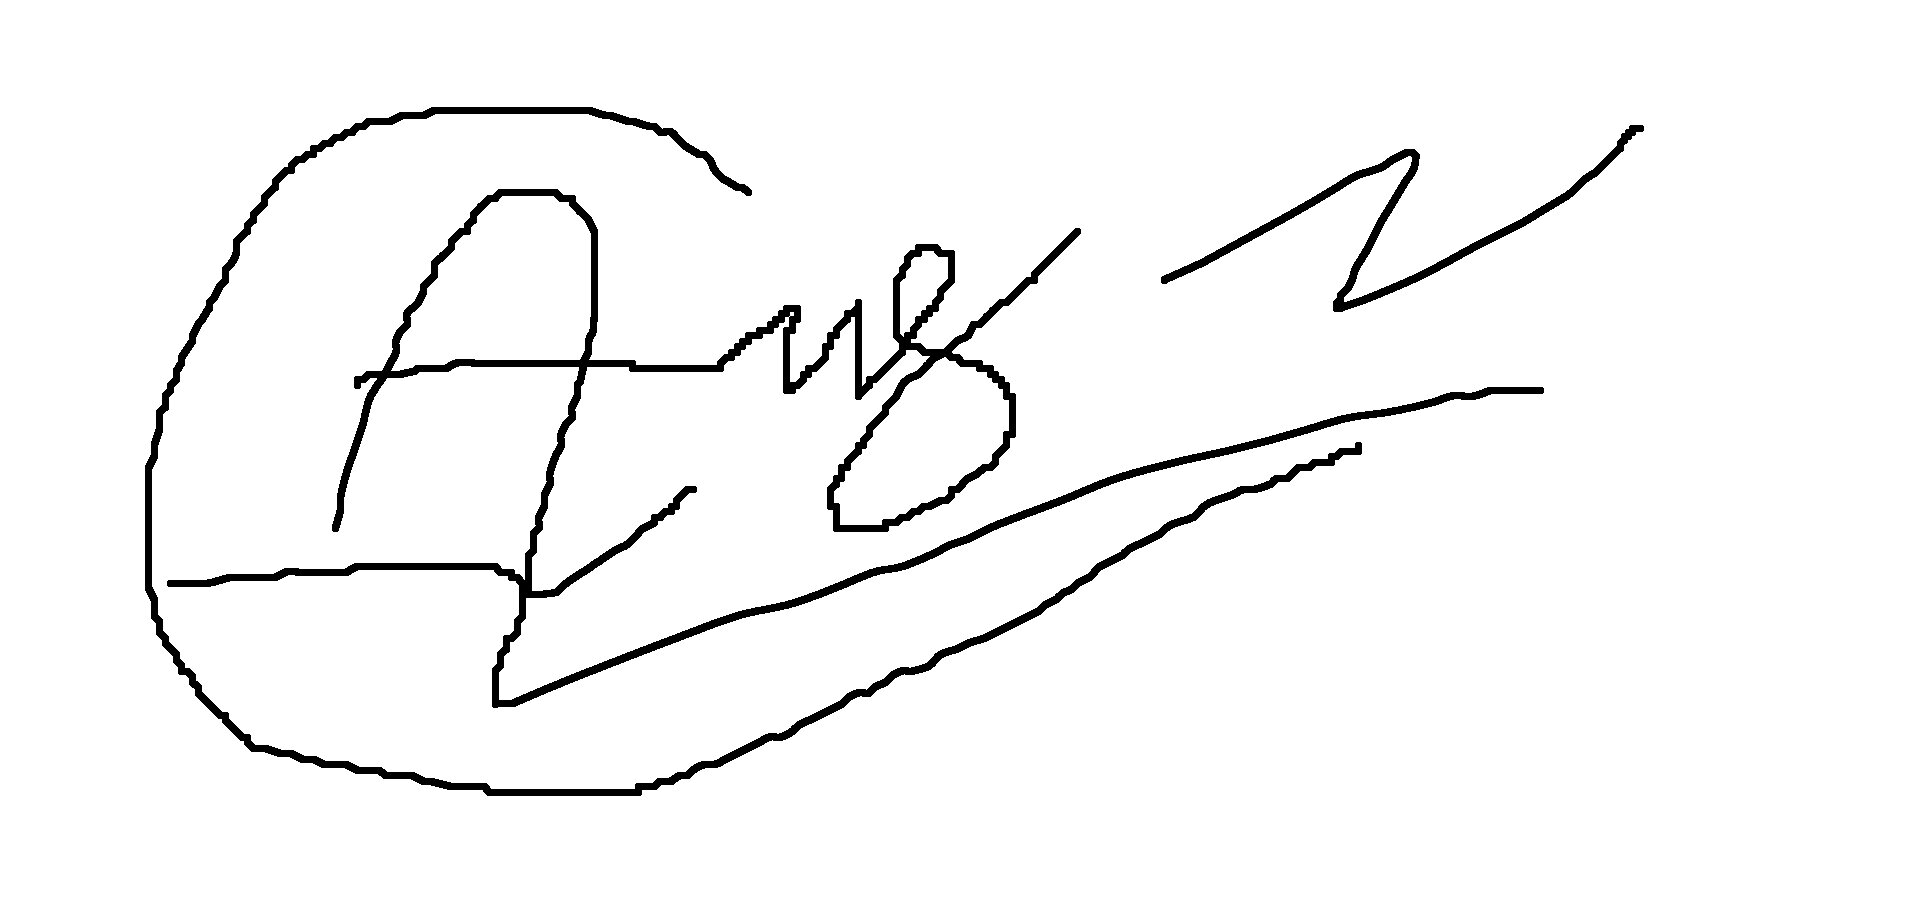
\includegraphics[width=\linewidth]{sig.jpg}
    \end{minipage}
    \rule{150pt}{1.5pt}\\
    (Подпись)\\[20pt]

    \textbf{Проверил:}\\[5pt]
    Ищенко Алексей Петрович\\[20pt]
    \rule{150pt}{1.5pt}\\
    (Отметка о выполнении)\\[20pt]
    \rule{150pt}{1.5pt}\\
    (Подпись)\\[55pt]
\end{flushright}
%\fancyfoot[C]{Текст в нижнем колонтитуле первой страницы}
\begin{center}
    Санкт-Петербург\\[3pt]
    2024 г.
\end{center}




\newpage
\begin{center}
    \tableofcontents
\end{center}





\newpage

\section{Техническое задание}

Написать программу, реализующую два исторических примера алгоритмов шифрования. Продумать интерфейс, руководство пользователя и описание работы алгоритмов (их историей и криптоустойчивостью), для демонстрации алгоритмов пользователю со встроенными примерами текстов (шифруем и дешифруем), а также с возможностью ввода произвольного текста с его шифровкой дешифровкой.

Для данной лабораторной работы надо разработать программу для ''Шифровка последовательностей нулей и единиц'', что было усложнено до XOR шифрования и ''Шифр Вижинера (для русских букв)''.

Необходимо реализовать следующие этапы для каждого алгоритма:
\begin{enumerate}
    \item Краткое описание алгоритма шифрования.
    \item Определение ограничений на решаемую задачу.
    \item Реализация данного алгоритма в виде программного кода.
    \item Реализация и описание графического интерфейса.
    \item Оформление отчета (включает описание выше и нижеизложенных пунктов со скриншотами работы программы и результатов).
\end{enumerate}


\section{Описание шифров}
\subsection{XOR}
XOR (исключающее ИЛИ) — простой симметричный шифр, основанный на применении побитовой операции XOR между символами исходного текста и ключа. Основные особенности:

\begin{itemize}
    \item Принцип работы: каждый символ текста преобразуется, используя соответствующий символ ключа (или ключ повторяется циклически).
    \item Шифрование и дешифрование идентичны: повторное применение операции XOR с тем же ключом восстанавливает исходное сообщение.
    \item Пример: для текста A (01000001 в бинарном виде) и ключа K (01001011), результат будет (00001010), что соответствует символу LF в ASCII.
    \item Применение: используется в простых системах шифрования, но уязвим для атак, если ключ короче текста или предсказуем.
\end{itemize}

\subsection{Шифр Виженера (для русских букв)}
Шифр Вижинера — это полиалфавитный шифр, использующий последовательность разных алфавитов для шифрования текста. Особенности его применения для русского алфавита:

\begin{itemize}
    \item Принцип работы: каждый символ текста сдвигается по алфавиту на число позиций, соответствующее символу ключа. Русский алфавит насчитывает 33 буквы, поэтому сдвиг выполняется циклически.
    \item Шифрование:
    \begin{itemize}
        \item Исходный текст: "ПРИВЕТ".
        \item Ключ: "КОД". (повторяется циклически: "КОДКОД").
        \item Результат:
        \begin{itemize}
            \item П + К = Т
            \item Р + О = Ф
            \item И + Д = Л
            \item и т.д.
        \end{itemize}
        \item Итоговый текст: "ТФЛЬЗФ".
    \end{itemize}
    \item Дешифрование: выполняется обратным сдвигом на число позиций ключа.
    \item Преимущества: стойкость выше, чем у простого шифра Цезаря.
    \item Недостатки: уязвим к частотному анализу, если ключ короткий.
    \item Этот шифр часто используется в учебных целях для изучения основ криптографии.
\end{itemize}

\section{Реализация и пример работы}
Весь код приведён в приложении к лабораторной работе

\subsection{XOR шифрование/дешифрование}
\textbf{Реализация}

Функция xor\_encrypt\_decrypt шифрует или дешифрует текст, используя XOR-операцию. Ключ применяется циклически, чтобы обработать весь текст. Каждая буква преобразуется с помощью побитового исключающего ИЛИ между её кодом ASCII и соответствующим кодом символа ключа.

\textbf{Пример работы}
\begin{itemize}
    \item Входные данные:
    \begin{itemize}
        \item Текст: hello
        \item Ключ: key
    \end{itemize}
    \item Шифрование:
    \begin{itemize}
        \item ASCII-коды текста: [104, 101, 108, 108, 111]
        \item ASCII-коды ключа (циклично): [107, 101, 121, 107, 101]
        \item Результат XOR: [3, 0, 21, 3, 10]
        \item Итоговая строка: ''\textbackslash x03\textbackslash x00\textbackslash x15\textbackslash x03\textbackslash n'' (защищённая форма текста).
    \end{itemize}
    \item Дешифрование:
    \begin{itemize}
        \item Применяя тот же ключ, исходный текст восстанавливается.
    \end{itemize}
\end{itemize}

\subsection{Шифр Виженера}

\textbf{Реализация}

Функция vigenere\_cipher использует алфавит из русских букв. В зависимости от режима работы (encrypt или decrypt), символы текста сдвигаются на позиции, определяемые соответствующими символами ключа.

Алгоритм шифрования:
\begin{enumerate}
    \item Для каждого символа текста находится его индекс в алфавите.
    \item Индексы символов ключа повторяются циклически.
    \item При шифровании символ текста сдвигается вперёд на количество позиций ключа.
    \item При дешифровании символ текста сдвигается назад.
\end{enumerate}

\textbf{Пример работы}

\begin{itemize}
    \item Входные данные:
    \begin{itemize}
        \item Текст: привет
        \item Ключ: ключ
    \end{itemize}
    \item Шифрование:
    \begin{itemize}
        \item Индексы текста: [16, 17, 8, 3, 5, 19] (позиции букв в русском алфавите).
        \item Индексы ключа (циклично): [10, 11, 23, 10, 11, 23].
        \item Результат: [26, 28, 31, 13, 16, 16] → Символы: ьфчкпп.
    \end{itemize}
    \item Итог: Зашифрованный текст — ьфчкпп.
\end{itemize}

\subsection{Пример работы программы}

Программа позволяет выбрать один из алгоритмов, режим работы (шифрование/дешифрование) и способ ввода текста (вручную или из файла). Результат выводится на экран или записывается в указанный файл.

Пример работы программы:

\begin{figure}[h!]
    \noindent
    \centering
    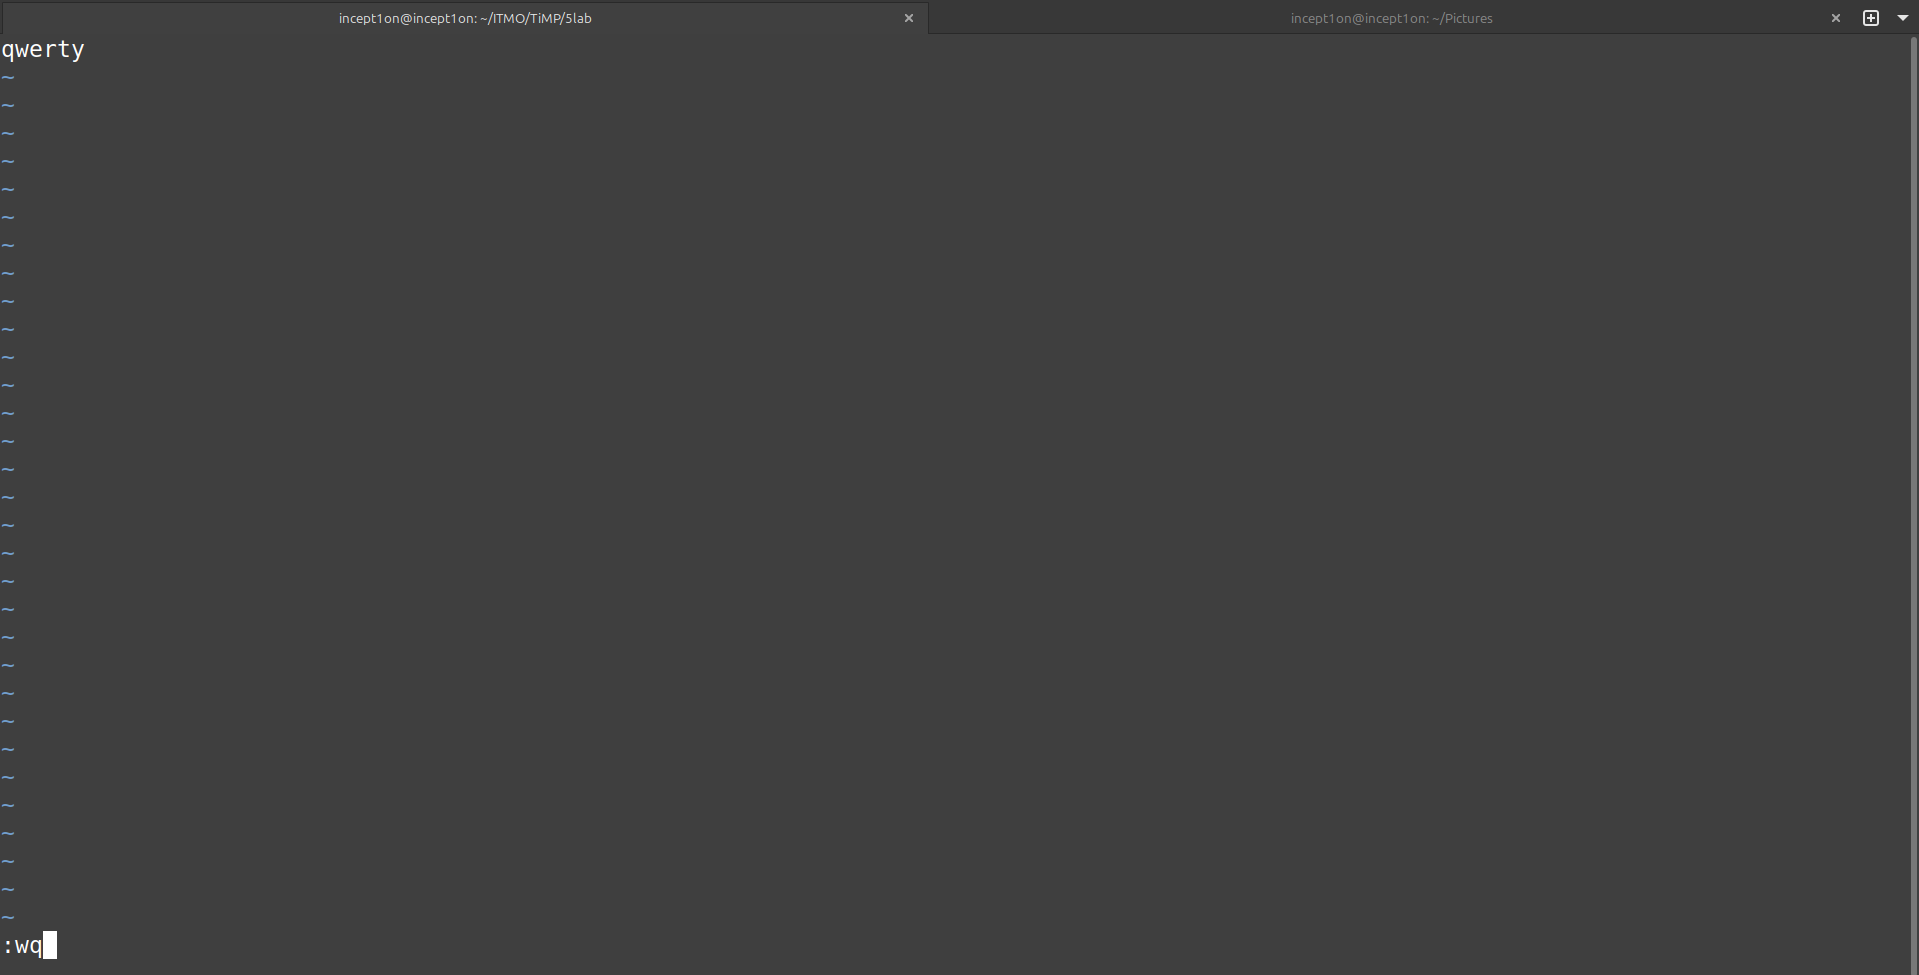
\includegraphics[width=1\linewidth]{pic_vim_create_file.png}
    \caption{Создаём файл, который будем кодировать с помощью XOR}
\end{figure}

\begin{figure}[h!]
    \noindent
    \centering
    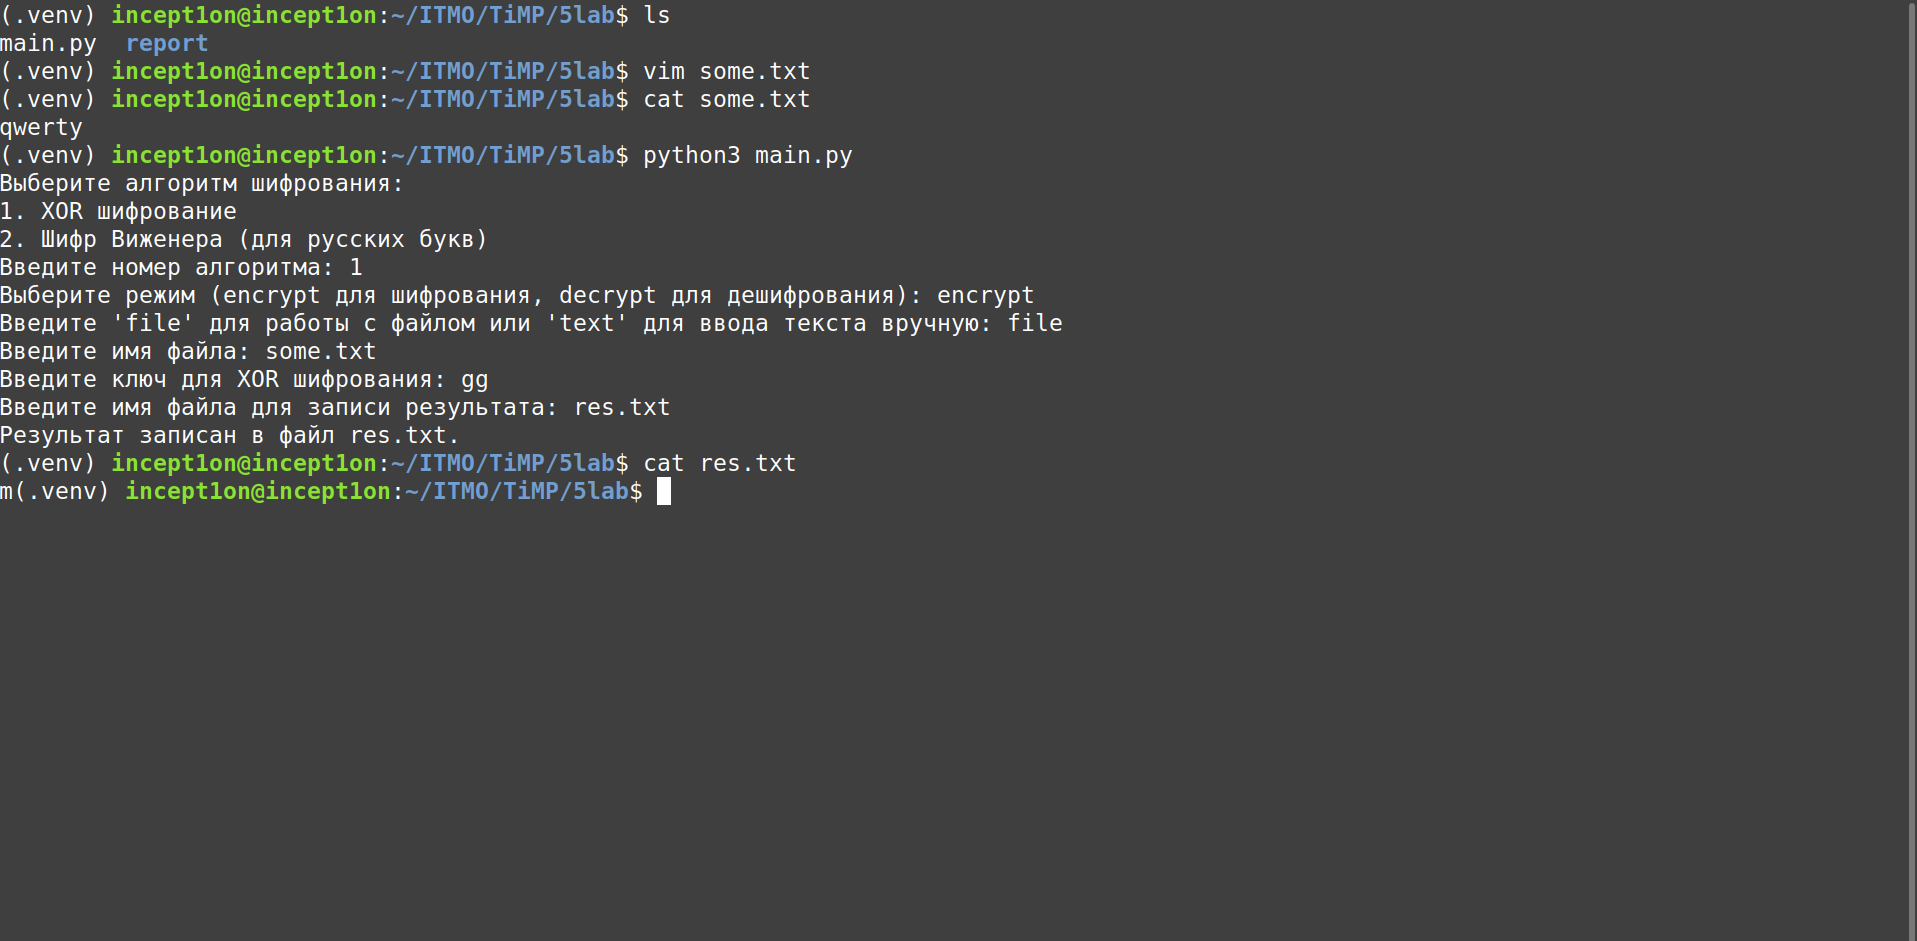
\includegraphics[width=1\linewidth]{pic_enc_xor.png}
    \caption{Шифруем файл}
\end{figure}

\newpage
Для сравнения покажем, как выглядят файлы в байтах, чтобы удостовериться, что всё зашифровано правильно. 

\begin{figure}[h!]
    \noindent
    \centering
    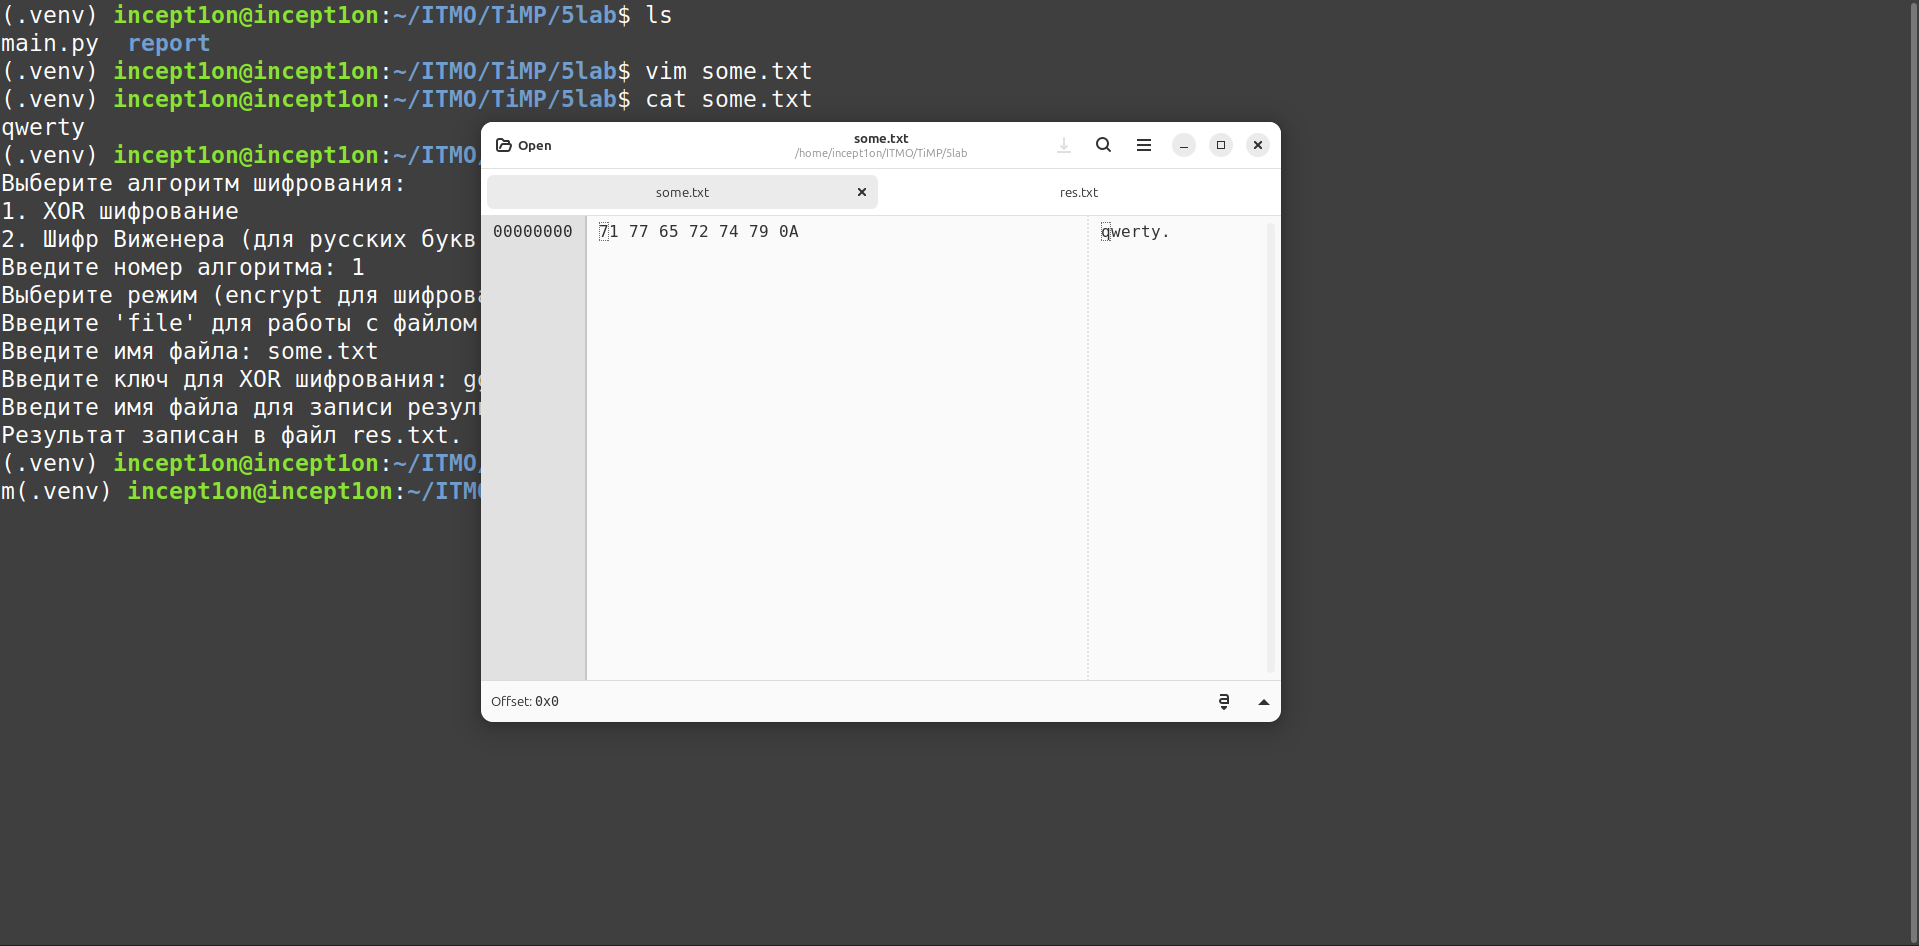
\includegraphics[width=1\linewidth]{pic_ghex_some.png}
    \caption{Файл some.txt}
\end{figure}

\begin{figure}[h!]
    \noindent
    \centering
    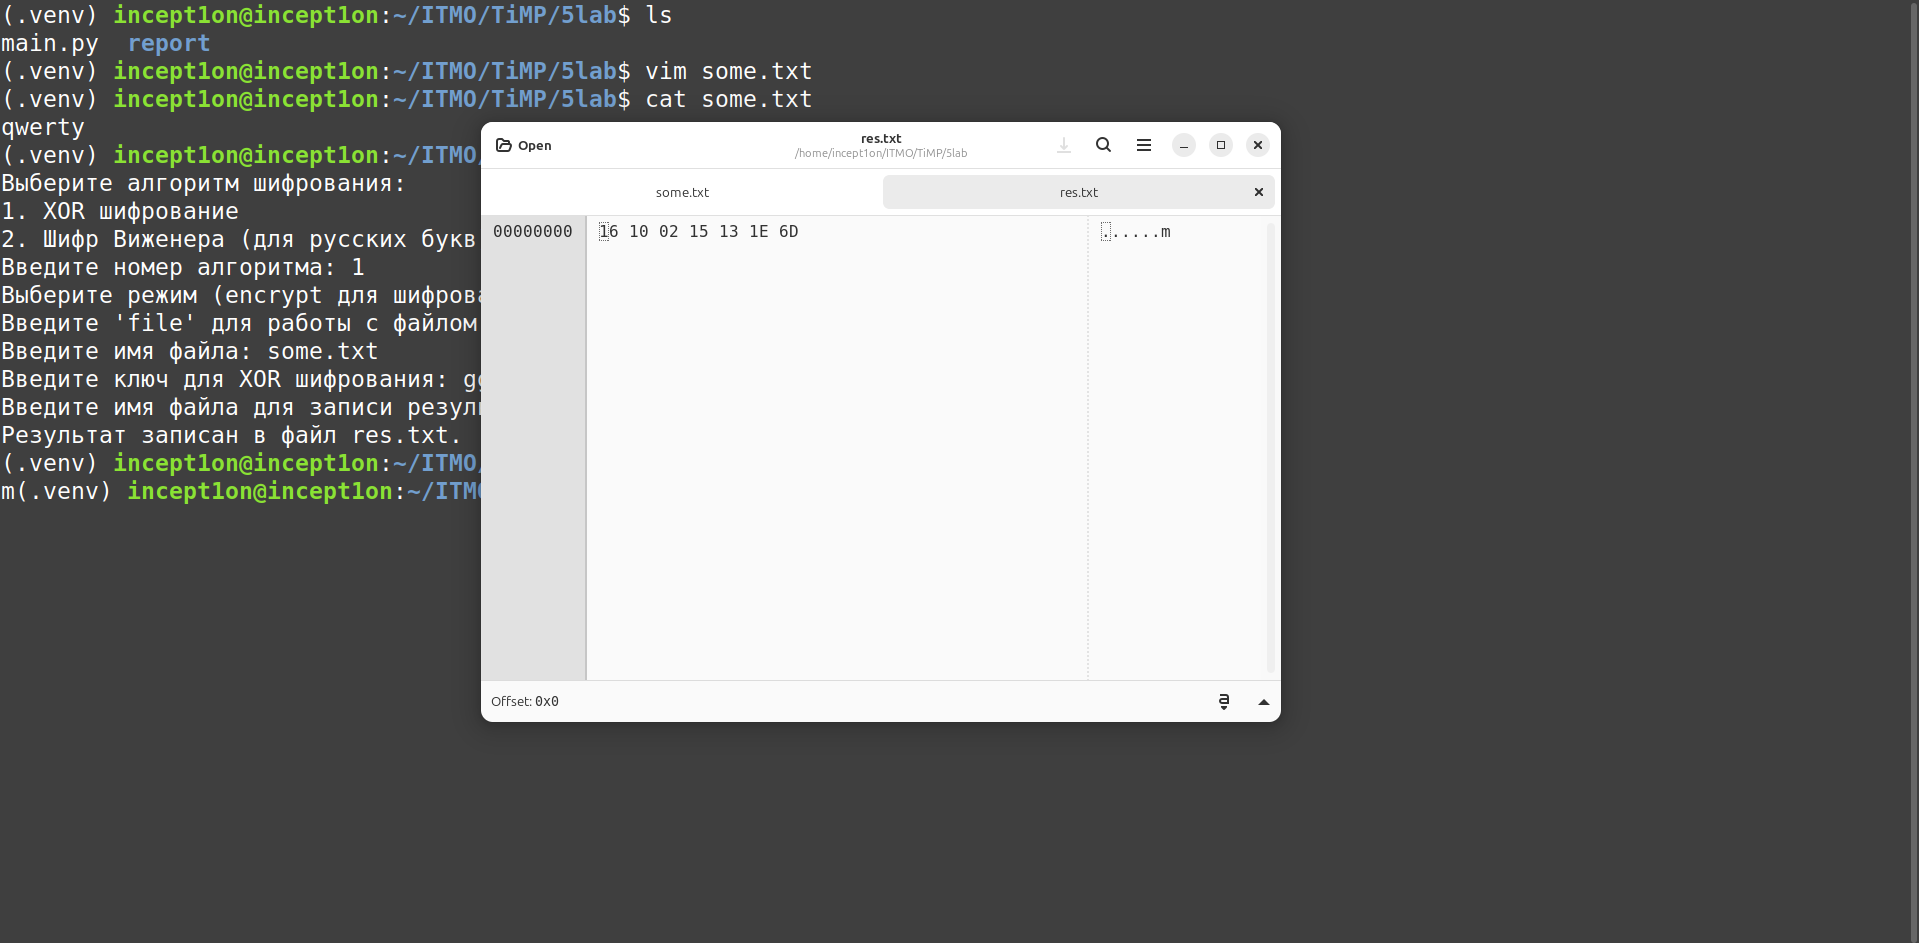
\includegraphics[width=1\linewidth]{pic_ghex_res.png}
    \caption{Файл res.txt}
\end{figure}

\begin{figure}[h!]
    \noindent
    \centering
    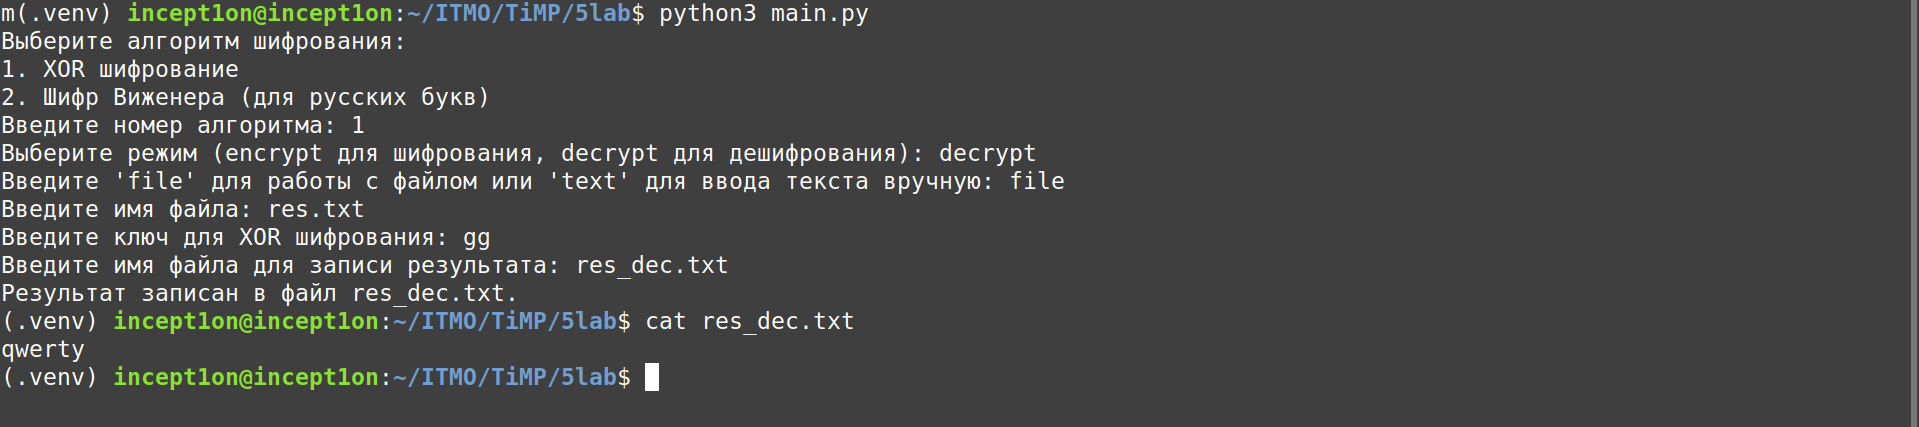
\includegraphics[width=1\linewidth]{pic_xor_decrypt.png}
    \caption{Расшифровка файла}
\end{figure}

\newpage    
\begin{figure}[h!]
    \noindent
    \centering
    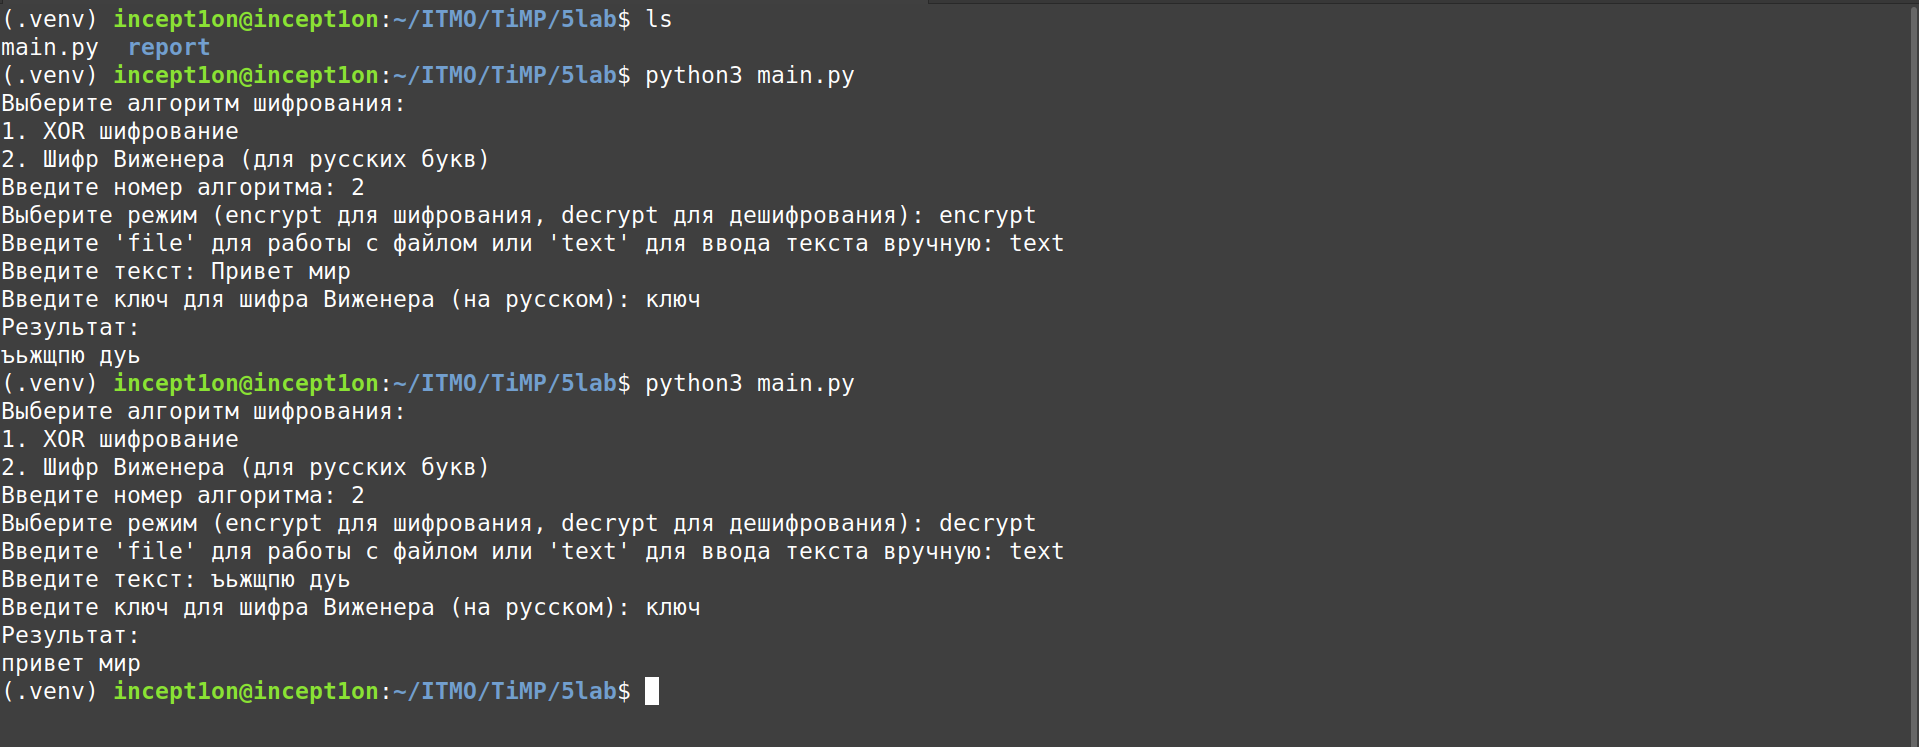
\includegraphics[width=1\linewidth]{pic_second_ciphr.png}
    \caption{Шифрование и расшифровка с помощью шифра Виженера}
\end{figure}




\newpage
\section{Заключение}
В ходе выполнения лабораторной работы были реализованы два исторических алгоритма шифрования: XOR и шифр Виженера для русского алфавита. Программа демонстрирует процесс шифрования и дешифрования, позволяя работать как с предустановленными примерами, так и с пользовательскими текстами.

Была проведена работа по следующим направлениям:
\begin{enumerate}
    \item Изучены принципы работы выбранных алгоритмов, их криптоустойчивость и ограничения. Для XOR характерна простота реализации, но низкая стойкость при использовании короткого или одноразового ключа. Шифр Виженера предоставляет более высокую устойчивость за счёт использования многоалфавитного подхода, но подвержен атаке Касиски при известных длинных текстах.
    \item Разработан программный код для шифрования и дешифрования текстов, включая поддержку русского языка.
    \item Создан удобный пользовательский интерфейс, обеспечивающий выбор алгоритма, режим шифрования/дешифрования, ввод текста и ключа, а также сохранение результатов в файлы.
    \item Реализованы встроенные примеры для демонстрации работы алгоритмов, что облегчает восприятие их принципов.
    \item Проведено тестирование программы, продемонстрирована её работоспособность на различных входных данных.
\end{enumerate}






\newpage
\section{Приложение}

\begin{lstlisting}[language=python, caption={Код для работы программы по шифрованию}]
import os


def xor_encrypt_decrypt(text, key):
    """
    XOR шифрование/дешифрование.
    """
    key_length = len(key)
    key_as_int = [ord(k) for k in key]
    text_as_int = [ord(t) for t in text]
    result = ''.join(chr(t ^ key_as_int[i % key_length]) for i, t in enumerate(text_as_int))
    return result


def vigenere_cipher(text, key, mode):
    """
    Шифр Виженера для русских букв.
    """
    alphabet = 'абвгдеёжзийклмнопрстуфхцчшщъыьэюя'
    result = []
    key = key.lower()
    key_indices = [alphabet.index(k) for k in key]

    for i, char in enumerate(text.lower()):
        if char in alphabet:
            char_idx = alphabet.index(char)
            key_idx = key_indices[i % len(key)]
            if mode == "encrypt":
                new_char = alphabet[(char_idx + key_idx) % len(alphabet)]
            elif mode == "decrypt":
                new_char = alphabet[(char_idx - key_idx) % len(alphabet)]
            result.append(new_char)
        else:
            result.append(char)

    return ''.join(result)


def read_from_file(filename):
    with open(filename, 'r', encoding='utf-8') as file:
        return file.read()


def write_to_file(filename, content):
    with open(filename, 'w', encoding='utf-8') as file:
        file.write(content)


def main():
    print("Выберите алгоритм шифрования:")
    print("1. XOR шифрование")
    print("2. Шифр Виженера (для русских букв)")
    choice = input("Введите номер алгоритма: ").strip()

    if choice not in {'1', '2'}:
        print("Неверный выбор. Завершение программы.")
        return

    mode = input("Выберите режим (encrypt для шифрования, decrypt для дешифрования): ").strip().lower()
    if mode not in {'encrypt', 'decrypt'}:
        print("Неверный режим. Завершение программы.")
        return

    source = input("Введите 'file' для работы с файлом или 'text' для ввода текста вручную: ").strip().lower()
    if source == 'file':
        filename = input("Введите имя файла: ").strip()
        if not os.path.exists(filename):
            print("Файл не найден.")
            return
        text = read_from_file(filename)
    elif source == 'text':
        text = input("Введите текст: ").strip()
    else:
        print("Неверный ввод.")
        return

    if choice == '1':
        key = input("Введите ключ для XOR шифрования: ").strip()
        if not key:
            print("Ключ не может быть пустым.")
            return
        result = xor_encrypt_decrypt(text, key)
    elif choice == '2':
        key = input("Введите ключ для шифра Виженера (на русском): ").strip()
        if not key.isalpha() or not all(c in 'абвгдеёжзийклмнопрстуфхцчшщъыьэюя' for c in key.lower()):
            print("Ключ должен содержать только русские буквы.")
            return
        result = vigenere_cipher(text, key, mode)

    if source == 'file':
        output_file = input("Введите имя файла для записи результата: ").strip()
        write_to_file(output_file, result)
        print(f"Результат записан в файл {output_file}.")
    else:
        print("Результат:")
        print(result)


if __name__ == "__main__":
    main()
\end{lstlisting}


\end{document}